\documentclass{article}
\usepackage[margin=1in]{geometry}
\usepackage{graphicx}
\usepackage{caption}
\usepackage{subcaption}
\usepackage{amsmath}
\usepackage{amssymb}

\title{Uncertainty Quantification for Satellite Image Segmentation}
\author{Mohamed Hasan}
\date{\today}

\begin{document}
\maketitle

\section{Introduction}
This report details the development and evaluation of a custom Artificial Neural Network (ANN) 
designed for image segmentation tasks. I focus on a UNet model architecture, built from scratch 
using TensorFlow 2, to perform segmentation on satellite images. To enhance the robustness and 
reliability of the model, I implement Monte Carlo (MC) Dropout as a method for uncertainty quantification. 
This approach allows me to assess the confidence of the model’s predictions, providing valuable 
insights into the reliability of segmentation results.
\vspace{1em}

The experiments involve an evaluation of different activation functions, loss functions, and 
other hyperparameters, with a focus on their impact on uncertainty quantification. The satellite 
image dataset, comprising of a mix of real and synthetic images and corresponding masks, serves as 
a challenging real-world scenario due to factors like variable lighting conditions, diverse backgrounds, 
and the presence of objects (i.e. astroids).


%%%%%%%%%%%%%%%%%%%%%%%%%%%%%%%%%%%%%%%%%%%%%%%%%%%%%%%%%%%%%%%%%%%%%%%%%%%%%%%%%%%%%%%%%%%%%%%%%%%%%%%%%%%%%%
\section{Dataset}
The dataset consists of satellite images and corresponding masks of size $1280 \times 720$, with each 
mask delineating the satellite from the background. The images are of varying resolutions and quality, 
reflecting the diversity of satellite imagery encountered in real-world scenarios. The dataset is divided 
into training and validation sets, with the training set containing 3117 images and the validation set
comprising 600 images. The masks are categorized into fine and coarse masks, with 403 fine masks
and 2114 coarse masks in the training set. The dataset presents a challenging segmentation task due
to the presence of complex textures, varying lighting conditions, and the need to accurately
delineate the satellite from the background.

\begin{figure}[h]
    \centering
    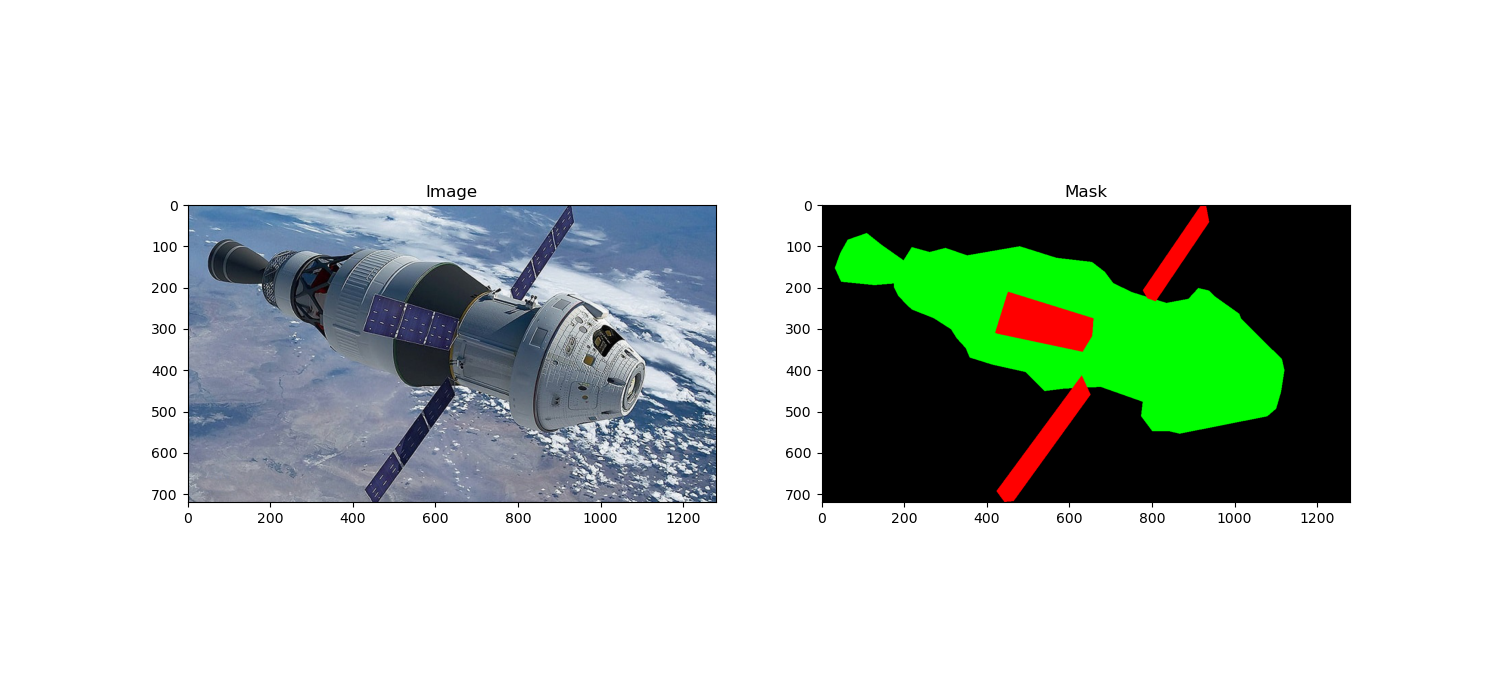
\includegraphics[width=0.8\textwidth]{../images/original_input_sample.png}
    \caption{Sample image and mask from the dataset. Image size is $1280 \times 720$.}
    \label{fig:original_dataset}
\end{figure}

\subsection{Data Preprocessing}

The dataset undergoes preprocessing to ensure uniformity and compatibility with the model. The images
are resized to a fixed resolution of $256 \times 256$ pixels and The masks are converted to binary format, with 
pixel values of 0 and 1 representing the background and satellite, respectively, to reduce computational
complexity. The preprocessed dataset has the same split between training and validation sets as the 
original dataset.
\vspace{1em}

The file \texttt{data\_loader\_unit.py} in the \texttt{utils} folder contains the function 
\texttt{load\_and\_process\_files()} to load the dataset and preprocess the images and masks. After processing, 
the data will be saved as numpy arrays for easy access during training. The saved files are named as follows:

\begin{itemize}
    \item \textbf{prepped\_data/trainimages.npy}: Contains the preprocessed training images.
    \item \textbf{prepped\_data/trainmasks.npy}: Contains the preprocessed training masks.
    \item \textbf{prepped\_data/valimages.npy}: Contains the preprocessed validation images.
    \item \textbf{prepped\_data/valmasks.npy}: Contains the preprocessed validation masks.
\end{itemize}
\vspace{1em}

The function to check if the prepped files exist is \texttt{check\_prepped\_data()} in the \texttt{utils} folder.
It is used in the scripts \texttt{train.py}, \texttt{predict.py}, and \texttt{main.py}. If the prepped files 
do not exist, the function is called to create them. Now, let's look at the processed dataset.

\begin{figure}[h]
    \centering
    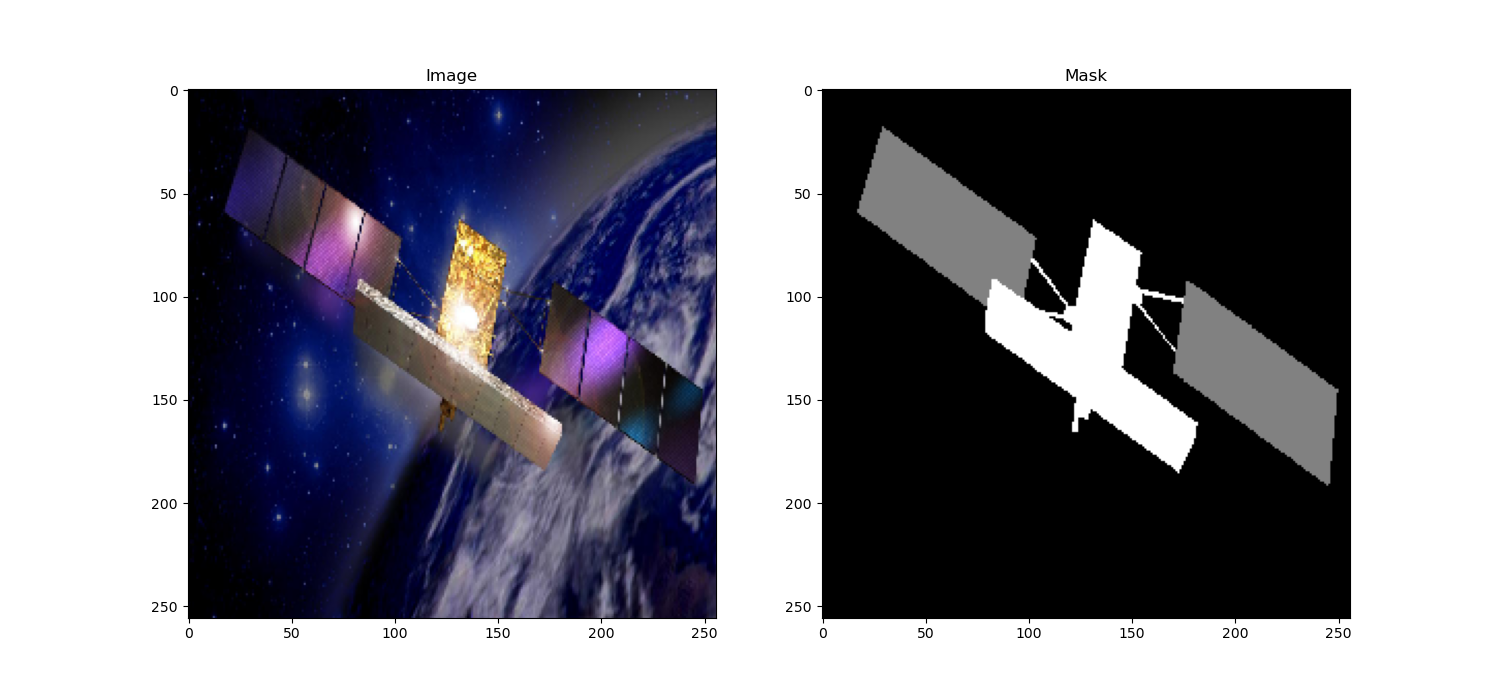
\includegraphics[width=0.9\textwidth]{../images/processed_input_sample.png}
    \caption{Sample processed image and mask from the dataset. Image size is $256 \times 256$ now and the mask is binary.}
    \label{fig:preprocessed_dataset}
\end{figure}


%%%%%%%%%%%%%%%%%%%%%%%%%%%%%%%%%%%%%%%%%%%%%%%%%%%%%%%%%%%%%%%%%%%%%%%%%%%%%%%%%%%%%%%%%%%%%%%%%%%%%%%%%%%%%%
\section{Model Architecture}
The model architecture is based on the UNet architecture, a popular choice for image segmentation tasks
due to its ability to capture both local and global features effectively. The model consists of an encoder
and a decoder, with skip connections between corresponding layers to preserve spatial information. The
encoder downsamples the input image to extract features, while the decoder upsamples the features to
generate the final segmentation map. The model is implemented using TensorFlow 2 and Keras, further
implementation details can be found in the model definition.

\begin{figure}[h]
    \centering
    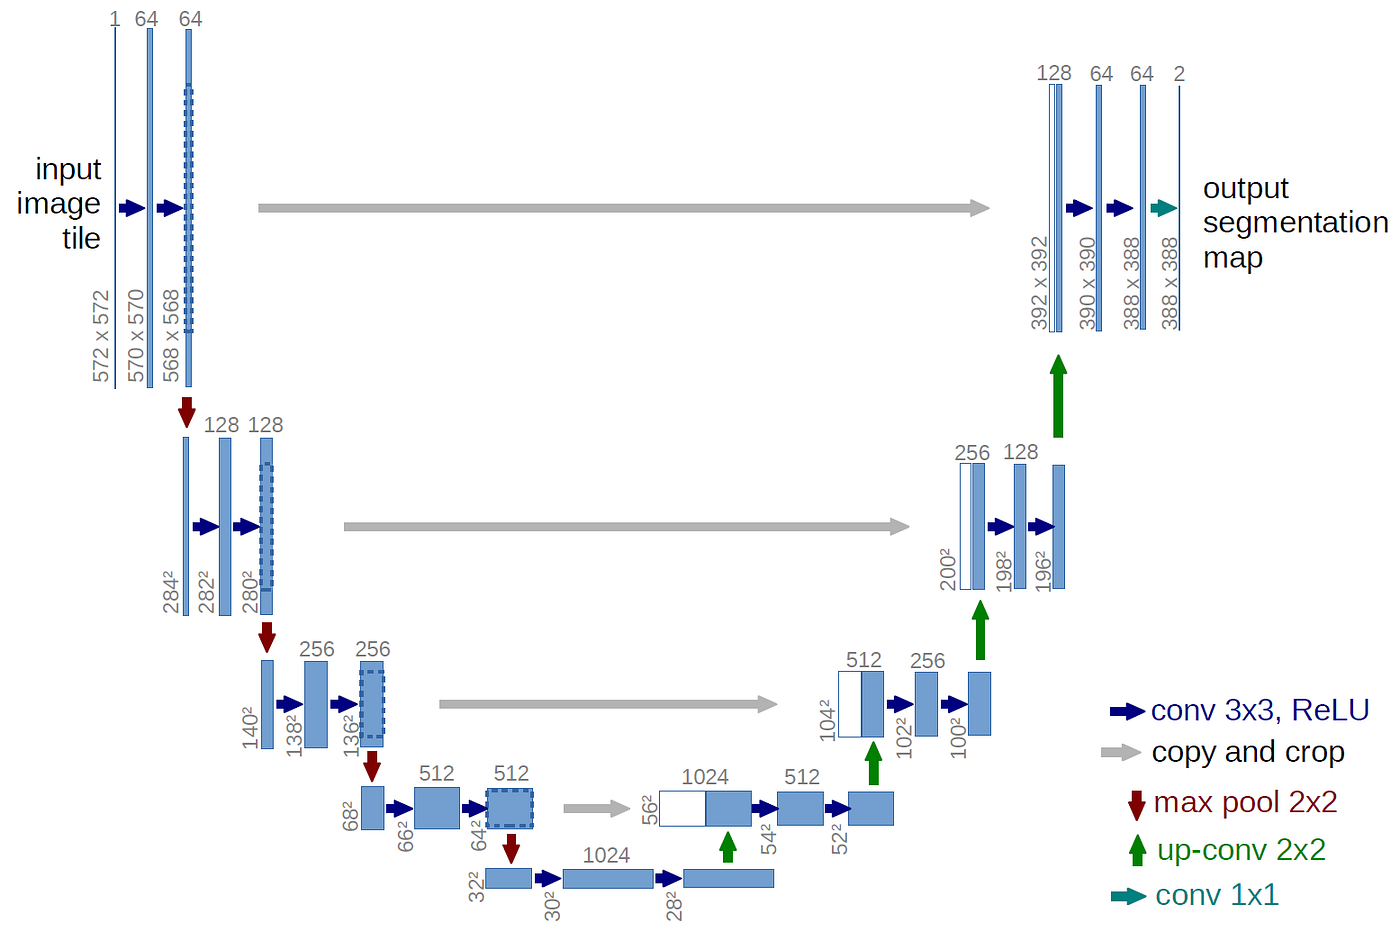
\includegraphics[width=0.9\textwidth]{../images/unet.png}
    \caption{Original UNet model architecture. We use a similar architecture with dropout layers for uncertainty quantification.} 
    \label{fig:unet_architecture}
\end{figure}
\vspace{1em}

The model architecture is defined in the file \texttt{unet.py} in the \texttt{model} folder. The implementation
is nearly identical to the standard UNet architecture. We add dropout layers after each convolutional layer
in the encoder and decoder, so that we may experiment with Monte Carlo Dropout for uncertainty quantification.

\subsection{Loss Function, Metrics, and Hyperparameters}

The loss function used for training the model is a combination of Binary Cross Entropy (BCE) and Dice Loss.
The BCE loss is effective in handling class imbalance, while the Dice Loss directly optimizes for the Dice
Coefficient, a common metric in image segmentation tasks. The Dice Coefficient is defined as

\[
\text{Dice Coefficient} = \frac{2 \times \text{Intersection}}{\text{Union} + \text{Intersection}} = 
\frac{2 \sum_{i=1}^{N} y_i p_i}{\sum_{i=1}^{N} y_i + \sum_{i=1}^{N} p_i},
\]

\[
\text{Dice Loss} = 1 - \text{Dice Coefficient},
\]

Where \( y_i \) is the ground truth label, \( p_i \) is the predicted probability, and \( N \) is the total 
number of pixels. The intersection is the number of overlapping pixels between the predicted and ground truth 
masks, and the union is the total number of pixels in both masks. The BCE loss is given by

\[
\text{BCE} = -\frac{1}{N} \sum_{i=1}^{N} [y_i \log(p_i) + (1 - y_i) \log(1 - p_i)],
\]

A combined loss function is used to leverage the strengths of both BCE and Dice Loss.

\[
\text{Combined Loss} = \text{BCE} + \text{Dice Loss}.
\]

The model is trained using the Adam optimizer with a learning rate of 0.001. The metrics used for evaluation 
are the Dice Coefficient and Accuracy.

\[
\text{Accuracy} = \frac{\text{Number of Correct Predictions}}{\text{Total Number of Predictions}}
\]
\vspace{1em}

The hyperparameters and model configurations are defined in the file \texttt{config.py} in the \texttt{model} folder.
The file contains the following hyperparameters:
 
\begin{itemize}
    \item \textbf{BATCH\_SIZE} = 1: The batch size used for training the model.
    \item \textbf{EPOCHS} = 5: The number of epochs for training.
    \item \textbf{DROPOUT\_RATE} = 0.35: The dropout rate used in the model.
\end{itemize}

\subsection{Evaluation}
The final model achieved:
\begin{itemize}
    \item Loss: 0.399
    \item Accuracy: 0.940
    \item Dice Coefficient: 0.803
\end{itemize}

The model shows good performance on the validation set, with high accuracy and Dice Coefficient, 
despite the challenging nature of the dataset and the low number of epochs. Let's visualize the model's 
predictions on a sample image from the validation set.

\begin{figure}[h]
    \centering
    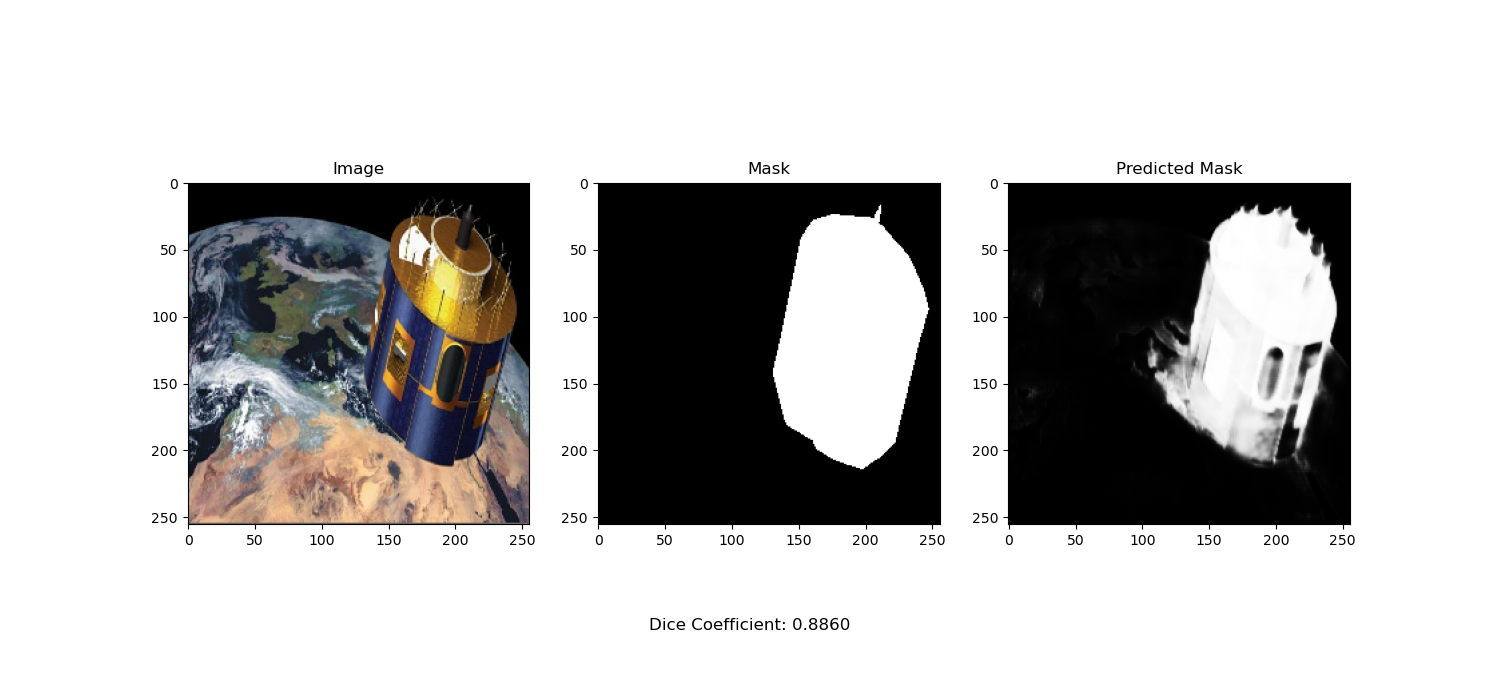
\includegraphics[width=0.9\textwidth]{../images/output_sample.png}
    \caption{Sample prediction from the validation set.}
    \label{fig:sample_predictions}
\end{figure}

The model successfully segments the satellite from the background, capturing the main features of the satellite
with a dice coefficient of 0.8860. Notice however that the model captures the details of the satellite which we 
did not include in the masks. This is due to the model's ability to learn from the training data and generalize.

%%%%%%%%%%%%%%%%%%%%%%%%%%%%%%%%%%%%%%%%%%%%%%%%%%%%%%%%%%%%%%%%%%%%%%%%%%%%%%%%%%%%%%%%%%%%%%%%%%%%%%%%%%%%%%
\section{Uncertainty Quantification}
\subsection{Monte Carlo Dropout}

For uncertainty quantification, I implemented the Monte Carlo (MC) Dropout technique. Dropout is a regularization method 
used during the training of neural networks to prevent overfitting. It works by randomly "dropping out" a subset of neurons 
during each forward pass, effectively creating an ensemble of different network architectures. Typically, dropout is 
disabled during inference to use the full capacity of the trained model. However, in MC Dropout, dropout is kept active 
during inference to introduce stochasticity into the model's predictions.

By incorporating dropout layers with a dropout rate of 0.35 during inference and performing multiple forward passes 
(in this case, 10 passes), I generated a distribution of predictions for each input image. This approach allowed me to 
capture the variability in the model's predictions due to the stochastic dropout, which can be interpreted as a measure of 
uncertainty.

The mean prediction for each pixel is calculated as follows:

\[
\mu(x) = \frac{1}{T} \sum_{t=1}^{T} \hat{y}_t(x),
\]

where \( \hat{y}_t(x) \) is the prediction at the \( t \)-th forward pass and \( T \) is the number of passes. The mean 
prediction provides an aggregate view of the model's output across multiple passes.

The uncertainty is quantified as the standard deviation of these predictions:

\[
\sigma(x) = \sqrt{\frac{1}{T} \sum_{t=1}^{T} (\hat{y}_t(x) - \mu(x))^2}.
\]

This standard deviation reflects the model's confidence in its predictions. A higher standard deviation indicates greater 
uncertainty, whereas a lower standard deviation suggests higher confidence. 

MC Dropout is particularly useful for identifying regions where the model is less certain about its predictions. In the 
context of image segmentation, uncertainty is often higher around the edges of objects and in regions with complex textures. 
This can be seen in Figure 5, where we can see the mean prediction and the standard deviation uncertainity generated by 
the MC Dropout technique for one of the validation images.

\begin{figure}[h]
    \centering
    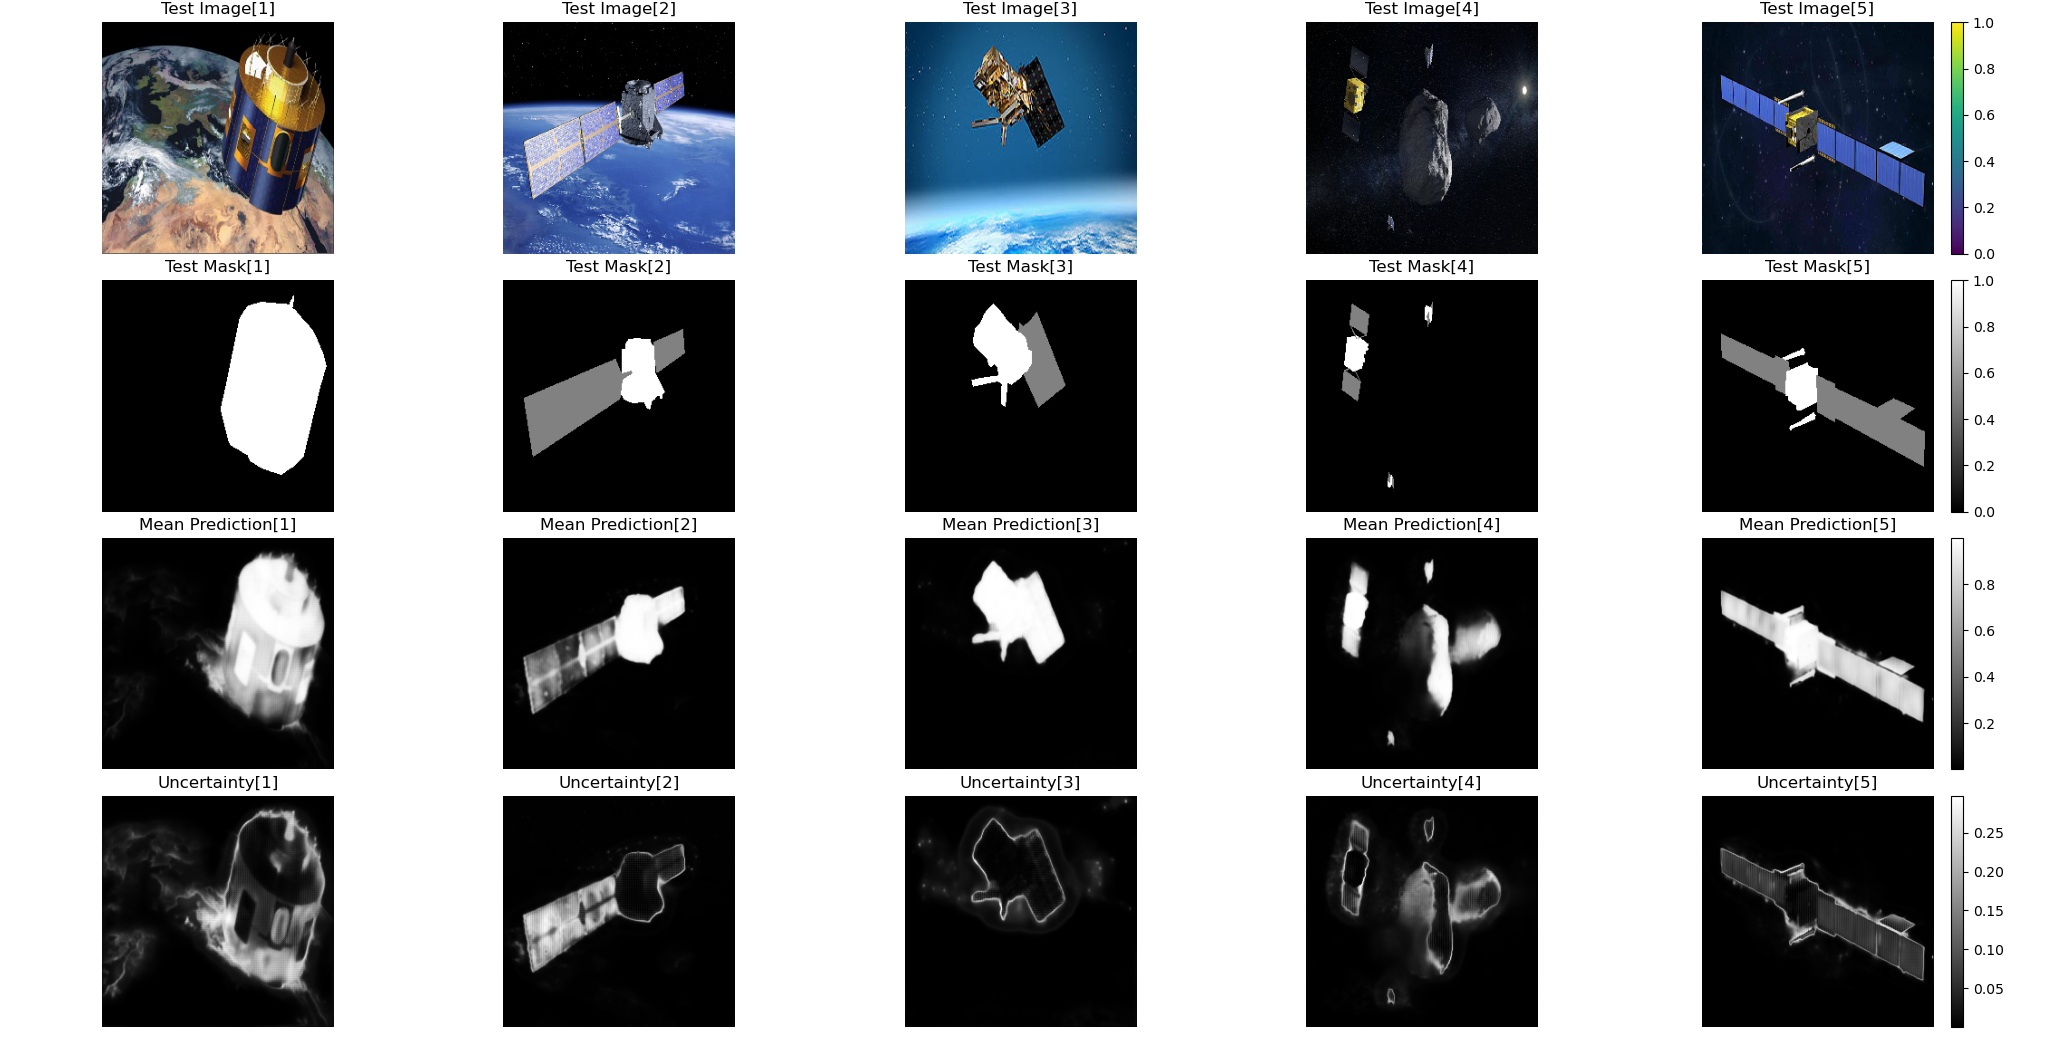
\includegraphics[width=0.9\textwidth]{../images/MC_dropout/test_image[0-5].png}
    \caption{We can see the test image, its mask, the mean prediction, and the uncertainty.}
    \label{fig:mc_dropout_single_image}
\end{figure}
\vspace{1em}

\begin{itemize}
    \item \textbf{test image[1]}: The satellite's body is well captured, but the model shows high uncertainty around the 
    edges and finer details. We can also see that the uncertainity makes sense, espeically near the bottom lower edge of 
    the satellite where there is a body of water. The water and the satellite are both blue in this case, so the model is 
    less certain about the prediction in that region.
    \item \textbf{test image[2]}: The satellite and its solar panels are identified, but the prediction is somewhat 
    spread, with significant uncertainty around the solar panels. This is most likely because the solar panels are blue 
    and the background is the blue oceans which makes it harder for the model to distinguish between the two.
    \item \textbf{test image[3]}: The satellite is identified quite well, with uncertainity only around the edges.
    \item \textbf{test image[4]}: The three satellites are identifies, but the model also identifes two astroids as satellites. 
    This is most likely due to the dataset not having many examples of astroids and the astroids having similar features 
    (most likely textures) to the satellites.
    \item \textbf{test image[5]}: The satellite is identified quite well, with uncertainity only around the edges.
\end{itemize}
\vspace{1em}



\end{document}
